\scanpage{164}
% archive sheet number: 163
% T1, landscape table, read by rows
\diagram{\begin{tikzpicture}
\node[inner sep=0] (t) {$\begin{array}{c|c|c|c|c|c|c|c|c}
&{\unsure{\mu|H}}_p&W_{11}&\mathbb Z/\unsure{\ell|l}\mathbb Z&\mathbb Z/p\mathbb Z&{\unsure{\mathbb G|G}}_m&\mathbb G_a&\mathrm{Ab}&\mathbb Z\\\hline
{}_p\mathbb G_m=\mu_p&\begin{gathered}\inserted{\text{par dualité}}\\\mathbb Z/p\end{gathered}&0&0* &*0&\deleted{\unsure{\mathbb Z/p}}0&0&\operatorname{Ext}(\mathbb G_m,{}_pA)&0*\\\hline
{}_F\mathbb G_a={\unsure{\mathbb W|W}}_{11}-&0&\mathbb G_a^2\ \text{\tikz[baseline=-.5ex]\node[draw,circle,inner sep=2pt]{?};}&0*&*0&0&\text{\tikz[baseline=-.5ex]\node[draw,circle,inner sep=2pt]{?};}&\operatorname{Ext}(\mathbb G_a,{}_pA)&0*\\\hline
\mathbb Z/\ell\mathbb Z&0*&0*&\mathbb Z/\ell\mathbb Z&0&\phi\ 0&\phi\ 0&\phi\ 0&\phi\ \mathbb Z/\ell\\\hline
\mathbb Z/p\mathbb Z&0*&0*&0&\mathbb Z/p\mathbb Z&\phi\ 0&\mathbb G_a&\phi\ 0&\phi\ \mathbb Z/p\mathbb Z\\\hline
\mathbb G_m&\mathbb Z/p\mathbb Z&0&\begin{gathered}\operatorname{Hom}(T(\mathbb G_m),\mathbb Z/\ell\mathbb Z)\\\simeq\mathbb Z/\ell\mathbb Z\end{gathered}&0\ \unsure{0|\circ}&0&0&\varinjlim\operatorname{Ext}(\mathbb G_m,{}_nA)&\\\hline
\mathbb G_a&0&\text{\tikz[baseline=-.5ex]\node[draw,circle,inner sep=2pt]{?};}&0\ \unsure{0|\circ}&\text{\tikz[baseline=-.5ex]\node[draw,circle,inner sep=2pt]{?};}&0&\text{\tikz[baseline=-.5ex]\node[draw,circle,inner sep=2pt]{?};}&\varinjlim\operatorname{Ext}^1(\mathbb G_a,{}_nA)&\smash{\text{\Huge ?}}\\\hline
\mathrm{Ab}&\multicolumn{4}{c|}{\operatorname{Hom}(T(A),G),\quad\unsure{h}}&(\mathrm{Ab})'&H^1(\mathrm{Ab},\underline{\unsure{\mathcal O|O}})&\deleted{\unsure{finis}}\ \text{----}&\\\hline
\mathbb Z&0*&0*&0*&0*&0*&0*&0*&0*
\end{array}$};
\draw ([xshift=-3pt,yshift=-20pt]t.north west) -- ++(-4pt,0) |- ([xshift=-3pt]t.west);
\draw ([xshift=-3pt,yshift=-3pt]t.west) -- ++(-4pt,0) |- ([xshift=-3pt]t.south west);
\end{tikzpicture}}

% L1-2, below table, left
$\phi\quad\operatorname{Ext}^1(\mathbb Z/n\mathbb Z,G)={}^nG$

\deleted{\unsure{donc}} $\operatorname{Ext}^1(F,G)=0$ si $F$ discret fini; $G$ divisible

% L3-7, below table, left
$*\quad$\unsure{deux groupes} \deleted{\unsure{finis}}, l'un \deleted{\unsure{étale}}\inserted{discret}, l'autre \unsure{radiciel|unipotent}, ont des ext. mutuelles nulles

% L8, outlined central heading
\figure{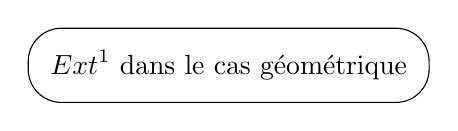
\begin{tikzpicture}\node[draw,rounded corners=12pt,inner sep=8pt] {$\operatorname{Ext}^1$ dans le cas \uline{géométrique}};\end{tikzpicture}}

% L9-10, heavily cancelled lower block
\deleted{N.B. $\operatorname{Ext}^2(\unsure{\mathbb G_a|\mathbb G_m},\mathbb G_m)\ne0$ \unsure{cf.} \illegible{4}}

% L11-12
\tikz[baseline=-.5ex]\node[draw,circle,inner sep=4pt]{?};\quad\uline{Consulter travaux Serre}

pour déterminations explicites

% Right-hand marginal note
\margin{Il n'est pas \unsure{clair} qu'il y ait lieu de considérer des ext. de $\mathbb G_a$, $\mathbb G_m$ ou $\mathrm{Ab}$ par $\mathbb Z$; on trouve \unsure{dans tous des} $0$}
